\chapter{Architectural Design}
\label{chap:architecture}

\section{Development Flow Stages}
\label{sec:top_level}

\begin{figure}[h]
\centering
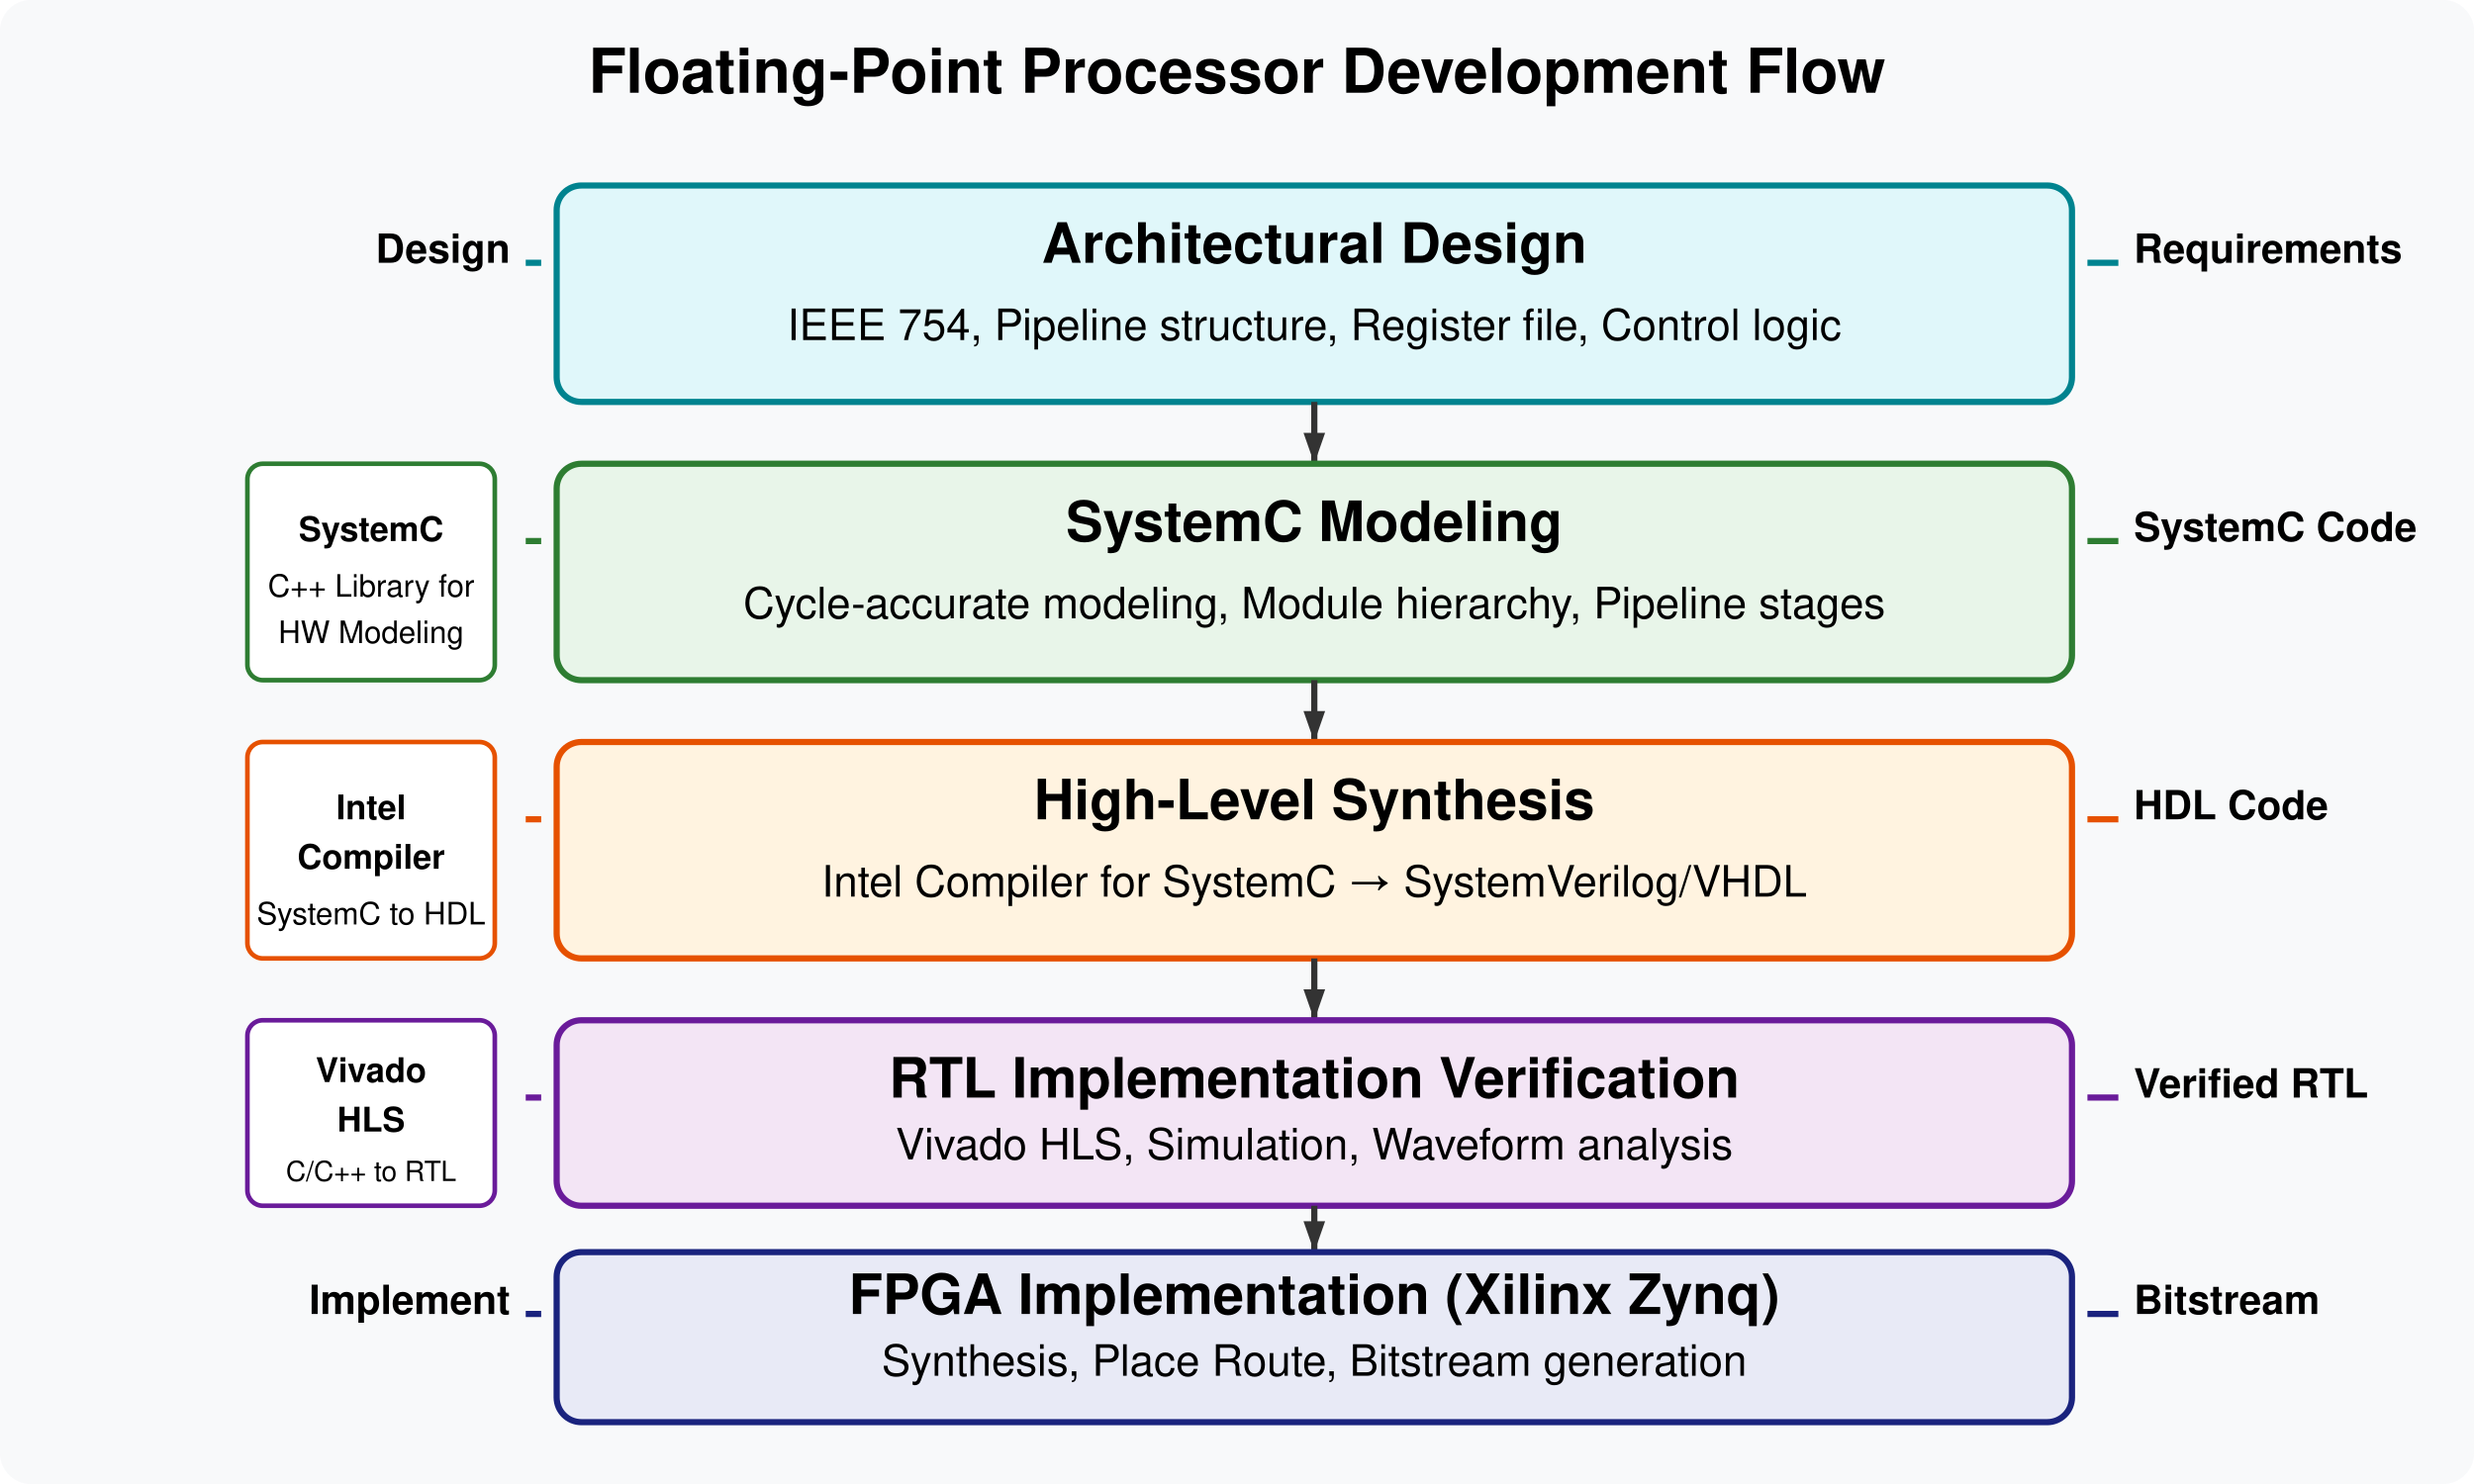
\includegraphics[width=0.8\textwidth]{figures/development.png}
\caption{Development flow stages of the pipelined floating-point processor}
\label{fig:top_level}
\end{figure}

\section{Design Requirements and Constraints}
\label{sec:design_req}

The floating-point processor design must satisfy the following functional requirements:

\begin{itemize}
\item Support for 32-bit single precision floating point format with 1 sign bit, 8 exponent bits, and 23 significand bits.
\item Implementation of addition, subtraction, multiplication and division operations with full precision.
\item Proper handling of special cases like zero, infinity, NaN and denormalised numbers.
\item Round to nearest (ties for even) to be implemented.
\item Handling exceptions like overflow, underflow, division by zero and invalid operations.
\end{itemize}

\section{IEEE 754 Floating-Point Standard}
\label{sec:ieee754_standard}

The IEEE 754 standard, formally known as IEEE Standard for Floating-Point Arithmetic, defines the technical details for floating-point computation. First published in 1985 and revised in 2008 (IEEE 754-2008), it has become the de facto standard for floating-point arithmetic in modern computing systems. This section provides a comprehensive overview of the standard's key aspects that directly influence the architectural design decisions of our pipelined floating-point processor.

\subsection{Standard Overview and Motivation}
\label{subsec:ieee754_overview}

Prior to IEEE 754, different computer manufacturers implemented floating-point arithmetic with varying formats, precision levels, and behavioral characteristics. This lack of standardization created significant portability issues for scientific and engineering applications. The IEEE 754 standard addresses these challenges by establishing:

\begin{itemize}
\item Standardized binary and decimal floating-point formats
\item Consistent rounding behaviors across different implementations
\item Uniform handling of special values and exceptional conditions
\item Predictable results for identical operations across different platforms
\end{itemize}

The standard ensures that floating-point operations produce identical results regardless of the underlying hardware implementation, provided both systems comply with IEEE 754 specifications.

\subsection{Floating-Point Number Representation}
\label{subsec:ieee754_representation}

IEEE 754 defines multiple precision formats, with single precision (binary32) being most relevant to our implementation. The mathematical representation of a floating-point number follows the formula:

$$(-1)^S \times (1 + M) \times 2^{E-bias}$$

Where:
\begin{itemize}
\item $S$ is the sign bit
\item $M$ is the significand (mantissa) representing the fractional part
\item $E$ is the stored exponent value
\item $bias$ is the exponent bias (127 for single precision)
\end{itemize}

\subsubsection{Single Precision Format (Binary32)}
\label{subsubsec:single_precision}

The 32-bit single precision format allocates bits as follows:

\begin{itemize}
\item \textbf{Bit 31:} Sign bit ($S$)
\item \textbf{Bits 30-23:} 8-bit exponent field ($E$)
\item \textbf{Bits 22-0:} 23-bit significand field ($M$)
\end{itemize}

The biased exponent representation allows for efficient comparison operations and eliminates the need for separate sign handling in the exponent. The bias value of 127 means that actual exponents range from -126 to +127, with stored values from 1 to 254 (0 and 255 are reserved for special cases).

\subsection{Special Values and Edge Cases}
\label{subsec:ieee754_special_values}

IEEE 754 defines specific encodings for special values that cannot be represented in the standard normalized format:

\subsubsection{Zero Values}
\label{subsubsec:zero_values}

Zero is represented with both exponent and significand fields set to zero. The standard defines both positive zero (+0) and negative zero (-0), distinguished only by the sign bit. These values are considered equal in comparisons but may produce different results in certain operations (e.g., division by zero).

\subsubsection{Denormalized Numbers (Subnormals)}
\label{subsubsec:denormalized}

When the exponent field is zero but the significand is non-zero, the value represents a denormalized number. These values use the formula:

$$(-1)^S \times (0 + M) \times 2^{1-bias}$$

Denormalized numbers provide gradual underflow, allowing representation of very small numbers that would otherwise underflow to zero. This feature maintains numerical stability in algorithms sensitive to small value precision.

\subsubsection{Infinity Values}
\label{subsubsec:infinity}

Infinity is represented with the exponent field set to all ones (255 for single precision) and the significand field set to zero. Like zero, infinity has both positive and negative variants. Infinity results from operations that exceed the representable range, such as division by zero or overflow conditions.

\subsubsection{Not-a-Number (NaN)}
\label{subsubsec:nan}

NaN values have the exponent field set to all ones and a non-zero significand. The standard defines two types of NaN:

\begin{itemize}
\item \textbf{Quiet NaN (qNaN):} Propagates through operations without raising exceptions
\item \textbf{Signaling NaN (sNaN):} Triggers an invalid operation exception when used in arithmetic operations
\end{itemize}

The most significant bit of the significand typically distinguishes between quiet and signaling NaN values.

\subsection{Rounding Modes}
\label{subsec:ieee754_rounding}

IEEE 754 defines five rounding modes to handle cases where the exact result cannot be represented in the target format:

\subsubsection{Round to Nearest, Ties to Even}
\label{subsubsec:round_nearest_even}

This is the default rounding mode, implemented in our processor design. When the result falls exactly between two representable values, rounding occurs toward the value with an even least significant bit. This approach eliminates systematic bias in repeated calculations.

\subsubsection{Round to Nearest, Ties Away from Zero}
\label{subsubsec:round_away_zero}

Similar to the previous mode, but ties are resolved by rounding away from zero rather than toward even values.

\subsubsection{Round Toward Zero (Truncation)}
\label{subsubsec:round_toward_zero}

Results are truncated toward zero, effectively discarding fractional portions. This mode never increases the magnitude of the result.

\subsubsection{Round Toward Positive Infinity}
\label{subsubsec:round_positive_infinity}

Results are always rounded toward positive infinity, useful in interval arithmetic applications.

\subsubsection{Round Toward Negative Infinity}
\label{subsubsec:round_negative_infinity}

Results are always rounded toward negative infinity, complementing the previous mode for interval arithmetic.

\subsection{Exception Handling}
\label{subsec:ieee754_exceptions}

IEEE 754 defines five types of floating-point exceptions that may occur during arithmetic operations:

\subsubsection{Invalid Operation}
\label{subsubsec:invalid_operation}

Occurs when an operation has no mathematically defined result, such as:
\begin{itemize}
\item Square root of a negative number
\item Addition of infinities with opposite signs
\item Multiplication of zero by infinity
\end{itemize}

The result is typically a NaN value.

\subsubsection{Division by Zero}
\label{subsubsec:division_by_zero}

Triggered when dividing a finite non-zero number by zero. The result is signed infinity.

\subsubsection{Overflow}
\label{subsubsec:overflow}

Occurs when the result magnitude exceeds the largest representable finite value. Depending on the rounding mode, the result may be infinity or the largest representable finite value.

\subsubsection{Underflow}
\label{subsubsec:underflow}

Happens when the result is too small to be represented as a normalized number. The result may be zero or a denormalized number, depending on the specific circumstances.

\subsubsection{Inexact}
\label{subsubsec:inexact}

Triggered when the result cannot be represented exactly and must be rounded. This is the most common exception in floating-point operations.

\subsection{IEEE 754 Compliance Requirements}
\label{subsec:ieee754_compliance}

For our processor to be IEEE 754 compliant, it must implement:

\begin{itemize}
\item Correct handling of all special values (zero, infinity, NaN, denormalized numbers)
\item Proper exception detection and reporting mechanisms
\item At least one required rounding mode (round to nearest, ties to even)
\item Consistent behavior for edge cases and boundary conditions
\item Correct sign handling for all operations and special cases
\end{itemize}

The architectural decisions in subsequent sections are designed to meet these compliance requirements while maintaining efficient FPGA implementation characteristics.

\section{Introduction to Architectural Design}
\label{sec:arch_intro}

This section describes the architectural design of a pipelined floating-point processor that balances IEEE 754 compliance with performance optimization and resource efficiency for Xilinx Zynq FPGA implementation. The design addresses pipeline hazards, ensures IEEE 754 compliant operations, and optimizes FPGA resources through critical components including exponent alignment, normalization, and rounding logic to achieve both accuracy and implementation efficiency \cite{ref16}.

\begin{figure}[h]
\centering
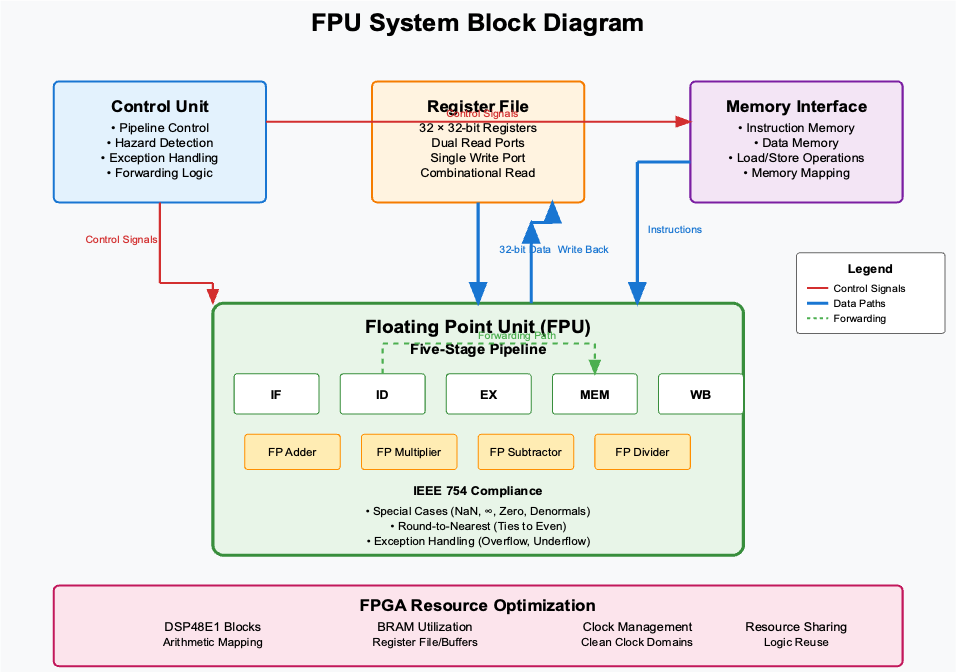
\includegraphics[width=0.8\textwidth]{figures/Con.png}
\caption{Control logic architecture of the pipelined floating-point processor}
\label{fig:control_logic}
\end{figure}

\subsection{Floating-Point Format and Representation}
\label{subsec:fp_format}

Building upon the IEEE 754 standard discussed in Section \ref{sec:ieee754_standard}, the processor implements the single-precision binary floating-point format with the following architectural considerations:

\begin{itemize}
\item \textbf{Sign Bit:} 1 bit indicating value sign (0 for positive, 1 for negative)
\item \textbf{Exponent:} 8 bits representing the biased exponent (actual exponent + 127)
\item \textbf{Significand:} 23 bits representing the fractional portion of the significand (with implicit leading 1 for normalized values)
\end{itemize}

Special values are encoded according to IEEE 754 conventions as detailed in Section \ref{subsec:ieee754_special_values}:

\begin{itemize}
\item \textbf{Zero:} Exponent = 0, Significand = 0 (signed)
\item \textbf{Denormalized Numbers:} Exponent = 0, Significand $\neq$ 0
\item \textbf{Infinity:} Exponent = 255, Significand = 0 (signed)
\item \textbf{NaN:} Exponent = 255, Significand $\neq$ 0
\end{itemize}

\subsection{Pipeline Structure}
\label{subsec:pipeline_structure}

The floating-point processor uses a five-stage pipeline architecture, based on the classic RISC-V pipeline structure modified for floating-point operations. The pipeline stages are:

\begin{enumerate}
\item \textbf{Instruction Fetch (IF):} Retrieves instruction from program memory
\item \textbf{Decode (ID):} Decodes instruction and reads operands from register file
\item \textbf{Execute (EX):} Performs floating-point operation (addition, subtraction, multiplication, division) with full IEEE 754 compliance
\item \textbf{Memory (MEM):} In this implementation, acts primarily as a pipeline register
\item \textbf{Writeback (WB):} Writes results back to register file
\end{enumerate}

This pipeline structure allows for efficient overlapping of instruction execution, with each stage processing a different instruction simultaneously, thereby maximizing throughput while maintaining precise IEEE 754 compliance as specified in Section \ref{subsec:ieee754_compliance}.

\subsection{Control Logic Design}
\label{subsec:control_logic}

The control logic is responsible for orchestrating all stages of the pipeline and for handling various hazards while ensuring IEEE 754 exception handling compliance:

\begin{itemize}
\item \textbf{Pipeline Stall Logic:} Helps pause the pipeline when required for multi-cycle operations or when hazards must be resolved
\item \textbf{Hazard Detection:} Operates to detect data hazards between instructions in the pipeline and determines the necessary handling routes
\item \textbf{Forwarding Logic:} Implements data forwarding to resolve data hazards without stalling the pipeline
\item \textbf{Exception Handling:} Detects and manages IEEE 754 exceptions (overflow, underflow, invalid operation, division by zero, and inexact) as defined in Section \ref{subsec:ieee754_exceptions}
\item \textbf{Special Value Detection:} Identifies and properly handles special IEEE 754 values during pipeline execution
\end{itemize}



\section{Register File Design}
\label{sec:register_file}

The register file is designed to support the IEEE 754 compliant floating-point operations:

\begin{itemize}
\item Support for 32 floating-point registers, each 32 bits wide for single-precision values
\item Dual read ports and single write port to maintain instruction throughput
\item Synchronous write operations on positive clock edge
\item Combinational read operations for minimal latency
\item Special value preservation through the register file to maintain IEEE 754 bit patterns
\end{itemize}

\section{Memory Interface}
\label{sec:memory_interface}

While this implementation focuses on floating-point processing pipelines rather than memory operations, the architecture includes:

\begin{itemize}
\item \textbf{Instruction Memory Interface:} For instruction fetching with proper IEEE 754 instruction encoding
\item \textbf{Data Memory Interface:} For loading and storing floating-point values while preserving IEEE 754 bit patterns
\item \textbf{Memory Mapping:} Appropriate address space allocation for floating-point data structures
\end{itemize}

\section{Design Considerations for FPGA Implementation}
\label{sec:fpga_considerations}

The architecture incorporates specific considerations for FPGA implementation while maintaining IEEE 754 compliance:

\begin{itemize}
\item \textbf{Efficient use of DSP blocks:} Arithmetic units are designed for effective mapping to DSP48E1 blocks while preserving IEEE 754 precision requirements
\item \textbf{Optimal memory resource utilization:} Register file and buffers are designed for efficient use of BRAM while maintaining IEEE 754 special value handling
\item \textbf{Pipeline depth optimization:} Pipeline depth is optimized to achieve target clock frequency while ensuring IEEE 754 operation completion
\item \textbf{Clock domain management:} Clean clock domain design with proper IEEE 754 exception propagation across domains
\item \textbf{Resource sharing:} Controlled resource sharing between operations requiring similar computations without compromising IEEE 754 compliance
\item \textbf{Special value optimization:} FPGA-optimized logic for detecting and handling IEEE 754 special values efficiently
\end{itemize}

The architectural decisions outlined in this chapter enable the SystemC implementation described in subsequent chapters to effectively map to both simulation environments and real-world FPGA hardware while maintaining full IEEE 754 standard compliance. The comprehensive IEEE 754 implementation ensures portability, predictability, and interoperability with other IEEE 754 compliant systems.